\chapter{About}
The primary goal of the project is to create a new platform for exploring, presenting, and supporting European visual art in virtual space.

Our vision emphasizes sustainability and leverages cutting-edge technologies like AI, virtual reality, and blockchain for long-term development.
Audience

The project caters to European visual artists, creators, galleries, collectors, curators, visitors, and art enthusiasts. Main focus: European visual art encompassing fine arts, photography, street art, video, etc.

\section{Innovations}

\subsection[3D]{Spatial 3D Gallery Environment}
The game like 3D environment allows artists to create their own exhibitions in a virtual space, providing a unique and immersive experience for visitors. The platform offers a variety of gallery environments to choose from, each with its own distinct style and atmosphere, enabling artists to curate their exhibitions in a space that complements their artwork.

For galleries and museums, the platform offers the possibility to create digital twins of their physical spaces or design entirely new digital environments for exhibitions, opening up new opportunities for showcasing art and engaging with audiences in innovative ways.

\subsection[NFT]{NFT Integration for Gallery Presentation}
The rise of digital art traded as NFTs has created a new market landscape, dominated by a few platforms like OpenSea. This project aims to bridge the gap between web3 NFT collections and traditional art, ensuring a seamless experience for both artists and digital gallery visitors.
AI Integration for Art Recognition and Browsing

\subsection[AI]{AI features for securing Art and improving the Browsing Experience}
The integration of advanced AI technology now facilitates the incorporation of smart tools capable of recognizing and categorizing art pieces. These tools significantly enhance the user experience by seamlessly navigating through extensive artistic collections and galleries. Users benefit from additional guidance and suggestions provided by the AI, streamlining the exploration process and enriching their interaction with art.
Referential implementation overview

Referential implementation integrates the minimum basic functionality of the virtual gallery environment.

\section{Target Audience}
The prototype accommodates the general functionality flows based on the user type and further decomposed in the requirements section:

\begin{itemize}
    \item \textbf{Visitors:}
        \begin{itemize}
            \item User-friendly experience emphasizing art presentation
            \item Public access to a diverse range of European art
            \item AI virtual assistant for discovering new art and staying updated on favorite artists and genres
        \end{itemize}
    \item \textbf{Artists:}
        \begin{itemize}
            \item Assembling of 3D virtual spaces for showcasing the art
        \item Utilization of blockchain technology for NFT digital art inclusion
        \end{itemize}
    \item \textbf{Galleries:}
        \begin{itemize}
            \item Creation of 3D digital twins or entirely new digital spaces for exhibitions
            \item Initial partnership with 1 main gallery in each member state, totaling 27 galleries initially
        \end{itemize}
\end{itemize}

\chapter{Features}

\section{Virtual Exhibitions}
Implementation of a 3D virtual gallery environment that allows artists to create and curate exhibitions in a digital space. The exhibitions can be customized with various gallery environments, providing a unique and immersive experience for visitors using a standard web browser. The exhibitions are viewed as an isolated environment within a browser and emulates a private exhibition experience without other visitors.
    \begin{itemize}
        \item \textbf{Spatial 3D web browser exhibitions:} The platform supports both NFT and non-NFT art, allowing artists to create mixed displays in a custom gallery prepared 3D environment. 
    \end{itemize}


\section{Blockchain Integration}
Implementation of the integration mechanism for the blockchain and NFT based art with the classical art world using novel technological approaches to art presentation and distribution. The blockchian extends the possibilities for artists to better present their art in front of a wider audience, as well as offer a new way of monetizing their work.

    \begin{itemize}
        \item \textbf{Wallet Integration:} Artists can connect their wallets to existing accounts or use them as primary accounts.
        \item \textbf{NFT art storage} Once connected, the entire NFT portfolio of the connected wallet is loaded, cached, tracked and synchronized with the Gallery account.
    \end{itemize}

\section{Art Theft Protection}
Implementation of a multi-layered approach to safeguarding artists' work, including:

    \begin{itemize}
        \item \textbf{Nightshade:} A cutting-edge technique~\cite{shan2024nightshade} that subtly alters artwork to render it useless for AI training while maintaining visual fidelity for human viewers.
        \item \textbf{NFT Minting:} Using blockchain technology to create NFTs for each artwork, ensuring verifiable authenticity and ownership.
        \item \textbf{Metadata Integration:} Leveraging standardized metadata formats to store essential information about the artwork, including artist attribution, ownership details, and licensing terms.
    \end{itemize}

\subsection{Protection from use in AI models}

Nightshade is a pioneering technique designed to protect artists' work from being exploited for training AI models. It introduces imperceptible perturbations to the image data, rendering it ineffective for AI training while preserving visual fidelity for human observers~\cite{shan2024nightshade}. This approach ensures that the artwork remains visually appealing and unaltered for human consumption, while effectively "poisoning" the data for AI algorithms.

\begin{figure}[ht]
    \centering
    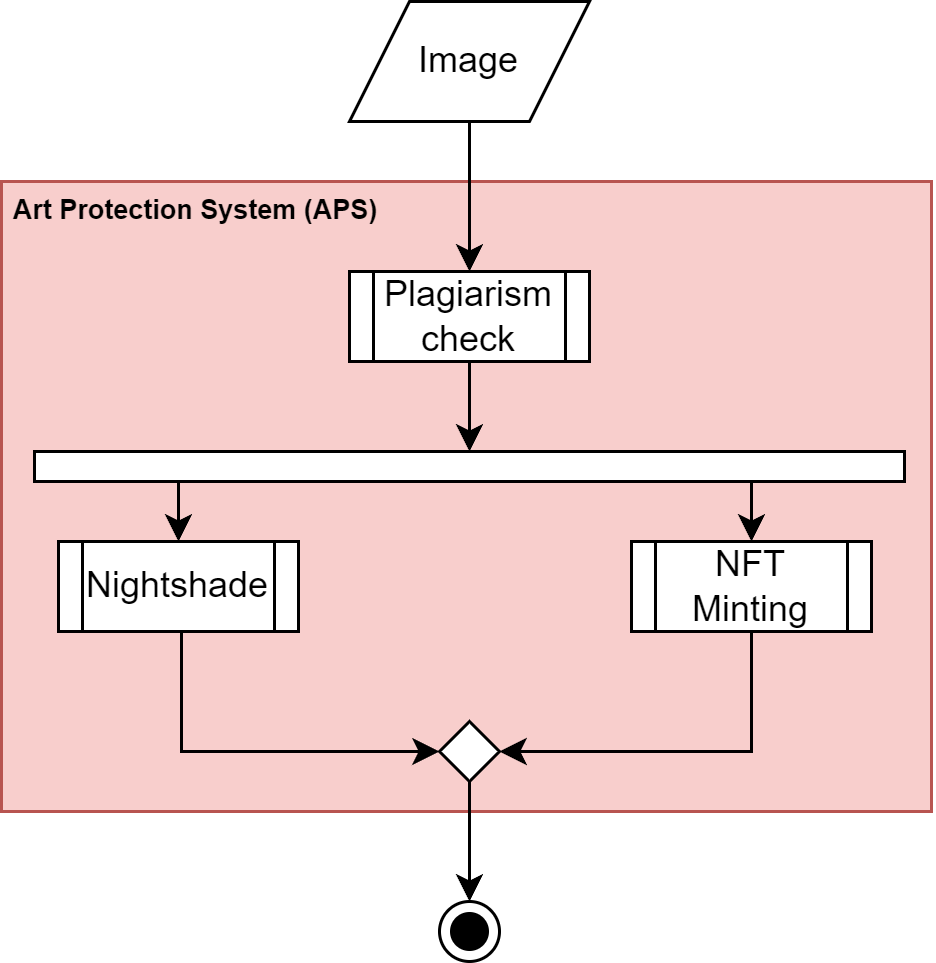
\includegraphics[width=0.8\textwidth]{figs/aps.png}
    \caption{Data flow through the processes for the Art Protection System in EVA Gallery.}
    \label{fig:data_flow}
\end{figure}

A similar tool, Glaze, focuses on protecting against style theft by subtly altering artwork to disrupt AI models' ability to mimic an artist's unique style~\cite{shan2023glaze}. However, Nightshade and Glaze are not yet interoperable, limiting their combined effectiveness in protecting against both content and style theft. EVA Gallery will monitor the development of these tools and integrate them when feasible to provide comprehensive protection against AI-powered art theft.

\subsection{Plagiarism check: a two-pronged approach}

EVA Gallery's plagiarism detection system employs a robust two-pronged approach to ensure the originality of uploaded artwork and protect artists' intellectual property rights, shown in~\autoref{fig:data_flow}.

\subsubsection{Embedding-based similarity check}

The first step involves converting the uploaded artwork into a high-dimensional numerical representation called an embedding. This embedding captures the semantic content of the image, including its objects, scenes, and overall meaning. The embedding is then compared against all existing embeddings in the database using efficient similarity search techniques like HNSW indexing. If an extremely close match is found, the artwork is flagged for further inspection.

\subsubsection{Gramian matrix similarity check}

Flagged images undergo a second level of scrutiny using Gramian matrix analysis. A Gramian matrix is a mathematical representation that captures the style of an image, including its textures, colors, and patterns. It is calculated from the feature maps extracted from the image by a pre-trained neural network.

Gramian matrices have been widely used in style transfer tasks, where the style of one image is transferred onto the content of another~\cite{nicolas2019improving}. However, their potential for style similarity comparison in the context of plagiarism detection is also promising. By comparing the Gramian matrix of the flagged image with those of existing artworks in the database, we can assess the degree of stylistic similarity. If a high match is found even at this stage, the artwork is flagged for human inspection.

This two-pronged approach provides a comprehensive check for plagiarism, considering both the semantic content and stylistic elements of the artwork. The embedding-based similarity check efficiently narrows down potential matches, while the Gramian matrix analysis delves deeper into the stylistic nuances to identify potential cases of plagiarism that may not be apparent from content alone.

By implementing this rigorous plagiarism detection system, EVA Gallery aims to create a fair and transparent platform where artists can showcase their work with confidence, knowing that their creations are protected from unauthorized copying and misuse.

\section{Plagiarism Protection}
Employ advanced techniques to detect and prevent plagiarism, ensuring the originality of uploaded artwork.

    \begin{itemize}
        \item \textbf{Embedding Space Lookup:} Artwork will be converted into numerical representations (embeddings) and compared within a vast database of existing art to identify potential copies or derivatives.
        \item \textbf{Gramian Matrix Similarity (Pending Research):}\footnote{Further research is needed to validate the effectiveness of this method for plagiarism detection.} A potential method that could further enhance plagiarism detection by analyzing the structural similarities between artworks.
        \item \textbf{Two-pronged Protection:} This system will guarantee that no modified artwork can be uploaded without proper attribution and permission, safeguarding artists' rights and fostering a fair creative environment.
    \end{itemize}

\section{Art Recommendation Engine}
Provide personalized recommendations to users based on their preferences and interactions with the artwork.

\begin{itemize}
    \item \textbf{Multi-Faceted Similarity:} Recommendations will consider both stylistic and content-based similarity to provide a diverse and engaging selection of artwork based on currently observed or displayed artwork.
    \item \textbf{Gramian-Based Style Recommendations:} Style-similar artwork will be evaluated using Gramian matrix similarity if proven viable.
    \item \textbf{Embedding-Based Content Recommendations:} Context-similar artwork will be displayed with respect to the typical similarity between embedded representations with MetaCLIP model.
    \item \textbf{Art Search:} Users will be able to input text that will be embedded and used to obtain images that most closely match the query.
\end{itemize}

\subsection{Embedding-based content recommendations}
EVA Gallery will take advantage of the power of image embeddings to provide content-based recommendations. By comparing the embedding of a user's observed artwork with the embeddings of other artworks in the database, we can identify pieces with similar semantic content, such as shared themes, subjects, or concepts. This enables us to recommend artworks that are similar to the currently observed artwork.

\subsection{Mixed recommendations (embeddings and Gramian matrices)}
To offer a diverse range of recommendations, we also consider a mixed approach that combines both embedding-based content similarity and Gramian matrix-based style similarity. This allows us to recommend artworks that share similar themes and visual styles with the observed artwork, providing a more comprehensive and engaging recommendation experience.

By incorporating both content and style information, we can cater to users who are interested in exploring artworks with similar subjects but different styles, or vice versa. This approach enhances the discovery aspect of the platform, exposing users to a wider array of artistic expressions.

\subsection{Gramian-based style recommendations}
For users who are primarily interested in visual styles, we offer recommendations based solely on Gramian matrix similarity. This allows us to identify artworks that share similar textures, colors, and patterns with the user's liked pieces, regardless of their semantic content.

This feature is particularly useful for users who are seeking inspiration for their own artistic creations or who are interested in exploring different artistic styles within a specific genre. By focusing on visual similarity, we can provide recommendations that corresponds best with the currently displayed artwork.

\chapter{User Stories}
Given the referential user types defined in the general overview, the expected user stories for the E.V.A. Gallery are:

\section{Website}
    \begin{itemize}
        \item The website should be optimized for speed and simplicity
        \item The website should use privacy non-intrusive storage to not force GDPR compliant pop ups
        \item The website is dynamically optimized for all device sizes (smartphone, tablet, laptop, large screen)
        \item The landing page contains the project logo
        \item The landing page contains a login option
        \item The landing page contains a search input
        \item The landing page contains an example query in the search input
        \item The exhibitions are rendered in browser
    \end{itemize}

\section{Visitor}
    \begin{itemize}
        \item The visitor access should not require login
        \item The visitor can access and browse individual art pieces directly or by URL
        \item The visitor can access and browse any artist collection directly or by URL
        \item The visitor can access and browse any gallery exhibition directly or by URL
        \item The visitor can view an artist profile with linked art, collections and exhibitions
        \item The visitor can search for an exhibition by its name
        \item The visitor can create an artist account to unlock the artist facing functionality
        \item The visitor's clicks and art browsing is recorded and used for further recommendations on the website
        \item The visitors are lightly fingerprinted to avoid overtraining the recommendation engine
    \end{itemize}

\section{Artist}
    \begin{itemize}
        \item The artist functionality is only available to registered users after login
        \item The artist can decide to have own account deleted
        \item The artist can create a public gallery exhibition
        \item The artist can remove own public gallery exhibition
        \item The artist can store and view own art items
        \item The artist can upload digital media representing the art items
        \item The artist can attach a web3 wallet to load NFTs
        \item The artist can choose any of the gallery environments to create an exhibition
        \item The artist can create multiple different exhibitions in the same gallery space each carrying a unique exhibition name
        \item The artist must assign a unique name to each exhibition in order to save it
        \item The artist can edit the exhibition once it is published
        \item The artist can delete the exhibition once it is published
    \end{itemize}


\chapter{Workflows}
\section{Data pipeline: Image upload and processing workflow}

Upon uploading an image to EVA Gallery, the system generates its embedding using the MetaCLIP model. This embedding captures the semantic content of the image and serves as the primary basis for content-based similarity search and recommendations.

The generated embedding is compared against all existing embeddings in the vector database using efficient similarity search techniques like HNSW indexing. If a close match is found, indicating potential plagiarism, the system extracts a Gramian matrix from either the encoded representation feature maps or from pre-computed matrices stored in the database. This Gramian matrix is then compared against the Gramian matrix of the uploaded image to assess the degree of stylistic similarity. If a high match is detected, the image is flagged for human review to determine whether it constitutes plagiarism. This and the whole pipeline is visualized in~\autoref{fig:pipeline}.

\begin{figure}[ht]
    \centering
    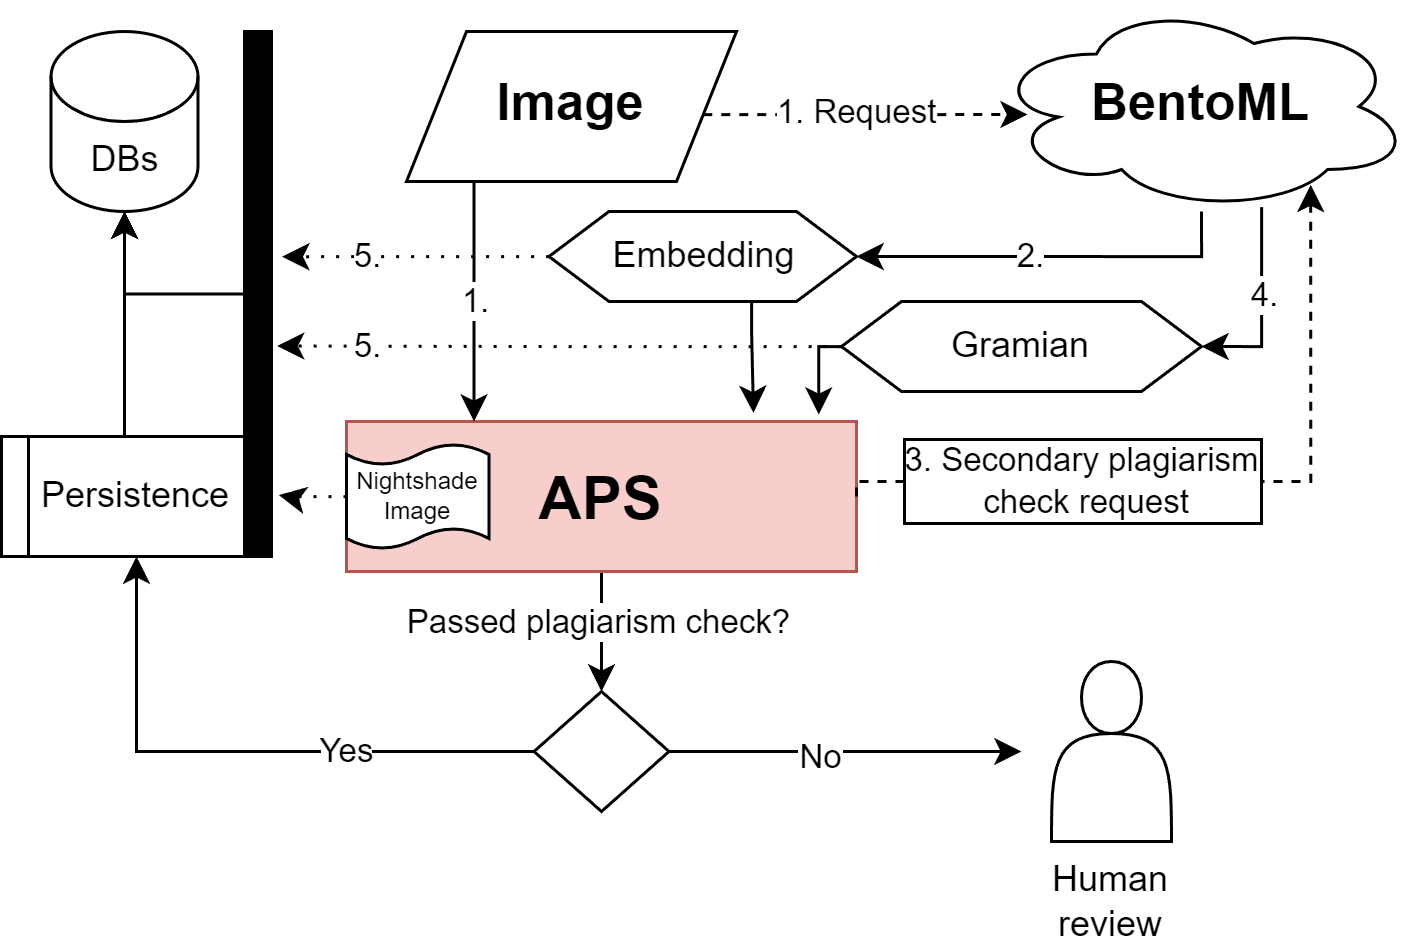
\includegraphics[width=0.8\textwidth]{figs/integ.png}
    \caption{Integration schema of the data pipeline, in other words, the image flow through the connected components of the system and the related infrastructure.}
    \label{fig:pipeline}
\end{figure}

Images that pass the plagiarism check are stored in the database along with their corresponding embeddings and Gramian matrices. Additionally, relevant metadata, including artist attribution, ownership details, and licensing terms, is associated with the image.

The artist has the option to mint the uploaded artwork as an NFT. The image is also processed with Nightshade, introducing subtle perturbations to render it useless for AI training while preserving visual fidelity. The Nightshade-processed image is stored as a separate copy in the database, linked to the original image via its unique UUID. This modified image is then displayed in the gallery, ensuring that visitors interact with the protected version while the original remains secure.

\newpage

\chapter{System Requirements}
\section{AI}
\begin{enumerate}
\item \textbf{Database Access:}
    \begin{itemize}
    \item Access to a database of existing images (UUID identified).
    \item Storage for modified images (Nightshade) alongside originals.
    \end{itemize}
\item \textbf{Vector Database:}
    \begin{itemize}
    \item Storage for embeddings and Gramian matrices.
    \item HNSW indexing for efficient similarity search.
    \end{itemize}

\item \textbf{Cloud Backend:}
    \begin{itemize}
    \item Hosts MetaCLIP (embeddings) and ResNet (Gramian matrices) models.
    \item Supports batched input.
    \item Simple API (e.g., BentoML).
    \end{itemize}

\item \textbf{Hardware Requirements:}
    \begin{itemize}
    \item MVP: GPU with at least 24GB VRAM.
    \item Deployment: Scalable GPU compute with load balancing and in-flight batching
    \end{itemize}
\end{enumerate}

\section{NFT}
\begin{enumerate}
    \item \textbf{Database Access:}
    \begin{itemize}
    \item Access to a database of existing images (UUID identified).
    \end{itemize}

\item \textbf{RPC provider:}
    \begin{itemize}
    \item Access to a RPC provider for the selected chain to fetch data from.
    \end{itemize}

\item \textbf{IPFS:}
    \begin{itemize}
    \item IPFS node where the NFT contents are typically located.
    \end{itemize}
\end{enumerate}

\section{Website}
\begin{enumerate}
    \item \textbf{Database Access:}
    \begin{itemize}
    \item Access to a database of existing images (UUID identified).
    \end{itemize}

\item \textbf{Frontend:}
    \begin{itemize}
    \item Scalable provider with frontend hosting capabilities.
    \item WASM support for 3D rendering.
    \end{itemize}

\item \textbf{Backend:}
    \begin{itemize}
    \item Scalable provider with backend hosting capabilities.
    \item Connectability for other services in the project.
    \item OAUTH enabled access
    \end{itemize}
\end{enumerate}

\newpage

\chapter{Technology stack}
\section{AI}

\begin{enumerate}
\item \textbf{Database Access:}
    \begin{itemize}
        \item \textbf{PostgreSQL:} A robust open-source relational database management system, offering support for structured data, ACID compliance, and scalability. Ideal for storing image metadata and maintaining associations between original and modified images.
        \item \textbf{Redis:} Local caching functionality for the frontend and backend, ensuring fast access to frequently accessed data.
    \end{itemize}

\item \textbf{Vector Database:}
    \begin{itemize}
        \item \textbf{pgvector+pgvectorscale+cube:} A PostgreSQL extension adding support for vector data types with similarity search using indexing algorithms, and matrix storage and search with cube. Cost-effective and scalable for storing and searching embeddings and Gramian matrices.
    \end{itemize}

\item \textbf{Cloud Backend:}
    \begin{itemize}
        \item \textbf{BentoML:} A flexible framework for building and deploying machine learning services. Simplifies packaging and deployment of models, allowing easy integration with various cloud providers, and supports batched input processing and API generation.
        \item \textbf{Self-hosted:} Kubernetes provides control and flexibility in configuring the software environment and automating deployment and building. We can utilize our existing servers with a proper MLDevOps architecture to ensure CI and CD alongside AI models.
        \item \textbf{IPFS instance:} Interactions with the NFT data stored in the Inter-Planetary FileSystem.
    \end{itemize}

\item \textbf{Scalable GPU Compute:}
    \begin{itemize}
        \item \textbf{Nvidia Triton Inference Server:} A high-performance inference server optimized for serving deep learning models. Supports dynamic batching and model ensemble, maximizing GPU utilization and throughput. Integrates with Kubernetes for seamless scaling and management.
    \end{itemize}
\end{enumerate}

\newpage

\chapter{API Specifications}
\section{NFT}
\begin{enumerate}
    \item \textbf{RPC Provider:}
    \begin{itemize}
        \item \textbf{Ethereum:} Infura, Alchemy, or similar providers for Ethereum-based chains.
        \item \textbf{Polygon:} Alchemy, QuickNode, or similar providers for Polygon-based chains.
    \end{itemize}

    \item \textbf{IPFS:}
    \begin{itemize}
        \item \textbf{IPFS HTTP API:} IPFS HTTP API for interacting with the IPFS node, including adding and retrieving NFT contents.
    \end{itemize}

    \item \textbf{Functionality:}
    \begin{itemize}
        \item abc
    \end{itemize}
\end{enumerate}
\newpage
\chapter{Choosing network for NFT infrastructure}
As many people know, the NFT(Non-fungible) market has been booming in recent years. This has led to a surge in interest from artists, collectors, and investors alike. However, the current infrastructure supporting NFTs is not without its challenges. One of the key issues facing the NFT market is the high gas fees associated with minting and trading NFTs on the Ethereum network. These fees can be prohibitively expensive, especially for smaller artists and collectors. As a result, many are looking for alternative networks that offer lower fees and faster transaction times.
We have observed available options which are as follows:
\begin{itemize}
    \item \textbf{Ethereum\footnote{Ethereum \url{https://ethereum.org/en/}}:} The most popular network for NFTs, but high gas fees and slow transaction times.
    \item \textbf{Polygon\footnote{Polygon \url{https://polygon.technology/}}:} A layer 2 scaling solution for Ethereum, offering low fees and fast transactions.
    \item \textbf{Gnosis chain\footnote{Gnosis chain \url{https://www.gnosis.io/}}:} A new blockchain network that aims to provide low fees and fast transactions for NFTs.
    \item \textbf{Polkadot\footnote{Polkadot \url{https://polkadot.network/}}:} A multi-chain network that aims to provide low fees and fast transactions for NFTs.
    \item \textbf{Solana\footnote{Solana \url{https://solana.com/}}:} A high-performance blockchain network that offers low fees and fast transactions.
\end{itemize}

We focused mostly on EVM chains as users are more likely to know Ethereum and have a wallet for it. We also considered Polkadot as it is a promising network with a lot of potential for future scalability, but Polkadot uses a different wallet address system with which users may not be as familiar. There is plenty of articles\footnote{Articles such as \url{https://webisoft.com/articles/best-blockchain-for-nft/}} about the best network for NFTs. Many research papers focus on non-fungible asset topics as well as comparisons of NFT infrastructure across different networks \cite{fintech1030017}.

To make precise and accurate decisions we need to consider the following factors:

\begin{itemize}
    \item Scalability of the network
    \item Availability of the tooling for NFT implementation and interaction with blockchain
    \item Programming language of the tooling
    \item Costs associated with creating collections and minting NFTs
    \item Speed of transactions
    \item Community support and adoption of NFT technology
    \item Environmental impact of the network
\end{itemize}

This data is compared across all mentioned networks in the table \ref{tab:networks}:

\begin{table*}[htb!]
    \caption{Comparison of various selected Blockchain Network parameters and NFT infrastructure}
\centering
    \begin{tabular}{|l|l|l|l|l|l|l|l|}
    \hline
    Network      & Scalability                                                                                                                                                                                          & Tooling                                                                                             & Prog. lang.                                                    & Avg. per NFT        & Block processing time & NFT adoption                                                                                                                                                     & Env. impact                                                                                                              \\ \hline
    Ethereum     & \begin{tabular}[c]{@{}l@{}}Often overloaded\\ when something \\ popular is released\\ (Drives GAS fees \\ up). 15-30 TPS \\ throughtput.\end{tabular}                                                & \begin{tabular}[c]{@{}l@{}}ERC721A standard \\ for cost optimization\end{tabular}                   & \begin{tabular}[c]{@{}l@{}}Solidity,\\ Javascript\end{tabular} & $\sim$$10 - $100+   & $\sim$12 seconds      & \begin{tabular}[c]{@{}l@{}}Very popular,\\ hosts some of \\ the most expensive \\ collections ever \\ made\end{tabular}                                          & \begin{tabular}[c]{@{}l@{}}After migrating\\ to PoS consensus\\ 99\% less\\ $\sim$2.8 kilotonnes\\ per year\end{tabular} \\ \hline
    Polygon      & \begin{tabular}[c]{@{}l@{}}Created as ETH\\ L2 chain to offlift\\ ETH. \\ $\sim$65000 TPS\end{tabular}                                                                                               & \begin{tabular}[c]{@{}l@{}}Crossmint API for \\ collection and nft \\ mint abstraction\end{tabular} & \begin{tabular}[c]{@{}l@{}}Solidity,\\ Javascript\end{tabular} & $\sim$$0.01 - $0.05 & $\sim$2.1 seconds     & \begin{tabular}[c]{@{}l@{}}Significantly lesser\\ adoption compared\\ to ETH, downtrend \\ in NFT adoption\end{tabular}                                          & \begin{tabular}[c]{@{}l@{}}$\sim$60.9 tonnes \\ per year\end{tabular}                                                    \\ \hline
    Gnosis chain & \begin{tabular}[c]{@{}l@{}}L2 solution hosted\\ by over 215.000\\ active validators\\ $\sim$155 TPS\end{tabular}                                                                                     & \begin{tabular}[c]{@{}l@{}}GoldRush to get\\ NFTs associated with\\ account\end{tabular}            & \begin{tabular}[c]{@{}l@{}}Solidity,\\ Javascript\end{tabular} & $\sim$$0.10 - $0.50 & $\sim$5 seconds       & \begin{tabular}[c]{@{}l@{}}Infrastructure strongly\\ tied to PoaPs, other\\ collections hardly\\ present\end{tabular}                                            & \begin{tabular}[c]{@{}l@{}}$\sim$25 tonnes\\ per year\end{tabular}                                                       \\ \hline
    Polkadot     & \begin{tabular}[c]{@{}l@{}}As multichain network\\ Polkadot is able to\\ disperse transactions to\\ different chains \\ (Up to 300 chains can \\ be in one network)\\ $\sim$100.000 TPS\end{tabular} & \begin{tabular}[c]{@{}l@{}}Substrate framework,\\ PolkadotJS libraries\end{tabular}                 & \begin{tabular}[c]{@{}l@{}}Rust,\\ Javascript\end{tabular}     & $\sim$$0.20-$1.30   & $\sim$12 seconds      & \begin{tabular}[c]{@{}l@{}}NFT infrastructure\\ well built but not\\ as utilized. Uses\\ different wallet \\ addresses (32B \\ compared to EVM 20B)\end{tabular} & \begin{tabular}[c]{@{}l@{}}$\sim$33 tonnes \\ per year\end{tabular}                                                      \\ \hline
    Solana       & \begin{tabular}[c]{@{}l@{}}Solana aims to be\\ one of the most \\ scalable blockchains \\ when it comes to TPS\\ $\sim$65000 TPS\end{tabular}                                                        & \begin{tabular}[c]{@{}l@{}}Compressed NFTs -\\ Minting 1.000\\ NFTs should cost 300\$.\end{tabular}  & Rust, C                                                        & $\sim$$3 - $4      & $\sim$0.6 seconds     & \begin{tabular}[c]{@{}l@{}}NFT adoption on\\ very strong level,\\ some collections\\ have more than \\ 130.000.000 eur \\ total volume\end{tabular}              & \begin{tabular}[c]{@{}l@{}}$\sim$8.875 tonnes\\ per year\end{tabular}                                                    \\ \hline
    \end{tabular}
    \label{tab:networks}
    \end{table*}


While Ethereum has the most documentation and tooling available, it also has the highest gas fees and slower transaction times. The Polygon chain excels at throughput, but the NFT infrastructure does not seem to be maturing. Gnosis chain is a new network with potential, but it lacks the community support and adoption of other networks. Solana's NFT ecosystem is also known for its revolutionary compressed NFT architecture which significantly reduces costs of minting.  Solana is a high-performance network with low fees, fast transactions, an eco-friendly orientation and a growing NFT infrastructure. Polkadot is a promising network with a lot of potential for future scalability, but it uses a different wallet address system that may be unfamiliar to users. Despite these facts, the NFT minting happens on-chain offlifting developers from creating and auditing smart contracts for NFT distribution. As the ecosystem is slowly growing we can expect, that the NFT adoption will rise as well. The tooling seems to also be sufficient enough for EVA Galery use cases. 